\documentclass[a4paper, 12pt]{article}
\usepackage[utf8]{inputenc}

%images
\usepackage{graphicx}       %for inserting images
\graphicspath{{../outputs/}}
\graphicspath{./}    %image file directory
\usepackage{wrapfig}
\usepackage{amsmath}
\usepackage{amssymb}
\usepackage{mwe}
\usepackage{listings} %for python code display
\usepackage{hyperref}	%hyperlink insertion
\usepackage{caption}	%caption

\captionsetup{
	font=small,
	labelfont=bf,
	tableposition=top
}
\usepackage{subcaption}	%for subfigures
\usepackage{geometry}
\geometry{margin = 0.7in}

%headers and footers
% All page numbers positioned at the bottom of the page
\usepackage{fancyhdr}
\fancyhf{} % clear all header and footers
\fancyfoot[C]{\thepage}
\fancyhead[R]{A. Thieshanthan, 180641N}   %header
\fancyhead[L]{\textbf{EN2550}}
\fancyhead[C]{Assignment A04}
\renewcommand{\headrulewidth}{1.5pt} % remove the header rule
\pagestyle{fancy}

%for inserting columns
\usepackage{multicol}       
\setlength{\columnsep}{1cm}

\usepackage{fancyvrb}
\usepackage{color}


%python code listing
\usepackage{listings}
\usepackage{xcolor}

\definecolor{codegreen}{rgb}{0,0.6,0}
\definecolor{codegray}{rgb}{0.5,0.5,0.5}
\definecolor{codepurple}{rgb}{0.58,0,0.82}
\definecolor{backcolour}{rgb}{0.95,0.95,0.92}

\lstdefinestyle{mystyle}{
	backgroundcolor=\color{backcolour},   
	commentstyle=\color{codegreen},
	keywordstyle=\color{magenta},
	numberstyle=\tiny\color{codegray},
	stringstyle=\color{codepurple},
	basicstyle=\ttfamily\footnotesize,
	breakatwhitespace=false,         
	breaklines=true,                 
	captionpos=b,                    
	keepspaces=true,                 
	numbers=left,                    
	numbersep=5pt,                  
	showspaces=false,                
	showstringspaces=false,
	showtabs=false,                  
	tabsize=4
}

\lstset{style=mystyle}

\usepackage[backend = biber, style = ieee]{biblatex}
\addbibresource{reference.bib}

%opening
\title{Assignment A04: Neural Networks}
\author{A. Thieshanthan, 180641N}

\begin{document}
	\maketitle
	\begin{abstract}
		This report covers the results and methods of implementing a Linear classifier, 2 Layer neural network and a convolutional neural network for  CIFAR-10 classification. Important parts of the code are provided within the report. Full code can be found at \url{https://github.com/thieshanthan/EN2550}.
	\end{abstract}
	\section{Linear Classifier}
		For this linear classifier, the scoring function $f(x)=Wx+b$ is used with the loss function Mean sum of squared errors(MSE). Some preparation and pre processing has been done to ease the coding and improve results. In some parts of the code numpy equivalent tensorflow functions are used to run the training on GPU.
		\subsection{Preparing dataset and Initializing parameters}
			The dataset images are normalized to produce a better effect on training. Normalizing is done by dividing by 255(largest entry in an image) and subtracting the mean of entire training set. Image labels are converted to one hot encoding vectors, which eases the loss computation. As there are 50000 training samples(m) with each image of size $32 \times 32\times 3$ the training dataset is reshaped into (3072, 50000) vector. This prepared dataset is used for Questions 1,2 and 3 of this assignment.
			\par 
			Weights $W$ and $b$ are initialized to random values as per standard normal distribution and zeros respectively. A dictionary $linear\_model\_history$ is initialized to store the history of training.
		\subsection{Model}
			As this is a simple model adding extra features such as learning rate decay, shuffling training data and adding regularization are relatively easy processes. For this model L2 regularization has been used. 
			
			\begin{multicols}{2}
				\noindent
				\begin{equation}
					\hat{Y}  = WX + b
				\end{equation}
				\begin{equation}
						L = \frac{1}{m}\sum{(\hat{Y}-Y)^2} - \frac{1}{m}\sum W^2
				\end{equation}
			\end{multicols}
			which results in following gradients,
			\noindent
			\begin{multicols}{2}
				\noindent
				\begin{align*}
					\frac{dL}{dw} &= \frac{2}{m}(\hat{Y} - Y)X^T - \frac{2}{m}W
				\end{align*}
				\begin{equation*}
					\frac{dL}{db} = \frac{2}{m}(\hat{Y} - Y)
				\end{equation*}
			\end{multicols}
		Using this gradients, gradient descent algorithm has been implemented. The backward propagation and gradient descent code is provided in listing \ref{backprop}
\begin{lstlisting}[language=python, caption=Backward Propagation and Gradient Descent, label=backprop] 
	# Loss function: Mean squared error loss
	loss = tf.math.reduce_sum((shuffled_y - y_hat)**2).numpy() / batch_size
	# Backward Pass
	dw1 = tf.matmul(y_hat - shuffled_y, shuffled_x, transpose_b=True) * (2/batch_size) 
	I = tf.ones((batch_size, 1))
	db1 = tf.matmul(y_hat - shuffled_y, I) * (2/batch_size)
	# Gradient descent
	w1 = w1 - learning_rate * dw1 - (reg)* w1
	b1 = b1 - learning_rate * db1
\end{lstlisting}
		\subsection{Training the classifier}
			Training has been done for 300 epochs with regularization and learning rate decay. Learning rate is reduced every 100 epochs and shuffling the training is also carried out. The hyperparameters and results are listed below in table \ref{param1}. The accuracy function used is provided in listing \ref{accuracy}
\begin{lstlisting}[language= Python, caption= Accuracy function used in Q1 Q2 and Q3, label=accuracy ]
def get_accuracy(y_hat, y):
	""" Classification accuracy  """
	y_hat_bin = np.argmax(y_hat,axis=0)
	y_class = np.argmax(y,axis=0)
	acc = 100*np.sum(y_hat_bin==y_class)/y_class.size
	return acc
\end{lstlisting}
			\begin{table}[h]
				\centering
				\begin{tabular}{|c|c|}
					\hline
					Hyperparameters & Value \\
					\hline
					Initial Learning rate & 0.0015 \\
					decay	& 0.001 \\
					regularization factor & 0.01 \\
					\hline
				\end{tabular}
				\caption{Hyperparameters for Linear Classifier}
				\label{param1}
			\end{table}
		\subsection{Results}
			\begin{table}[h]
				\centering
				\begin{tabular}{|c|c|c|c|c|}
					\hline
					epoch & Training Loss & Training accuracy & Testing loss & Testing accuracy\\
					\hline
					1 & 1.0050 & 10.49 & 0.9953 & 15.41 \\
					300 & 0.8702 & 30.42 & 0.8696 & 30.91\\
					\hline
				\end{tabular}
				\caption{Training and testing loss and accuracy for linear classifier}
			\end{table}
			The trained weights are displayed as 10 images in figure \ref{fig:weights} and graphs of losses and accuracy are presented in figure \ref{fig:ling}.
			\begin{figure}
				\centering
				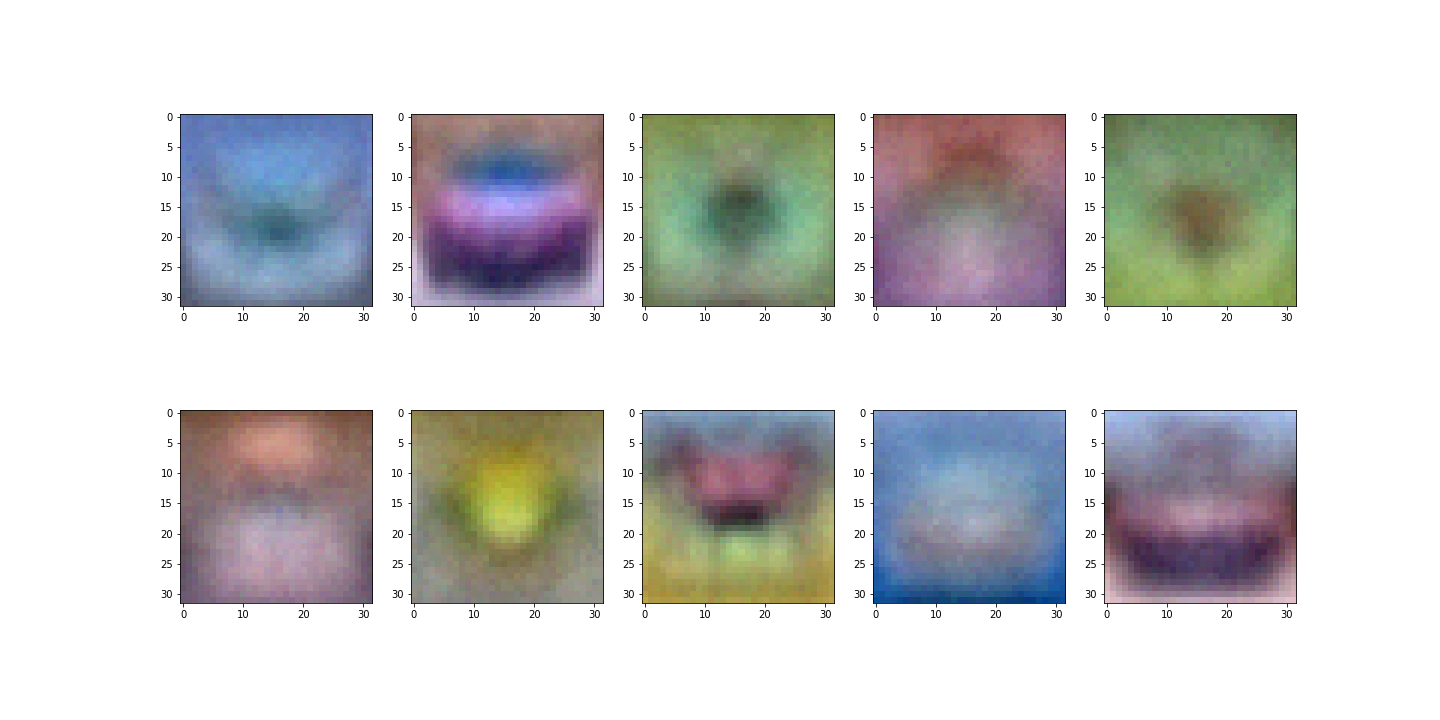
\includegraphics[scale = 0.4]{../images/weights}
				\caption{Trained weights of linear classifier}
				\label{fig:weights}
			\end{figure}
			\begin{figure}[h]
				\begin{subfigure}{0.45\linewidth}
					\centering
					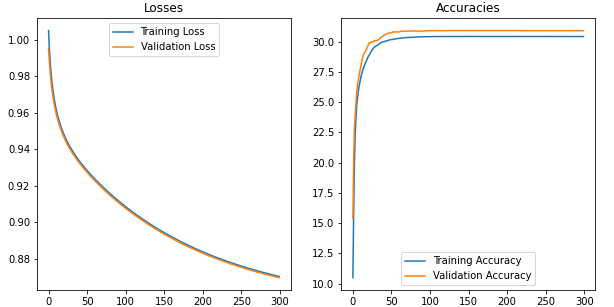
\includegraphics[scale = 0.35]{../images/linear_model}
					\caption{Training of linear classifier}
					\label{fig:ling}
				\end{subfigure}
				\hfill
				\begin{subfigure}{0.45\linewidth}
					\centering
					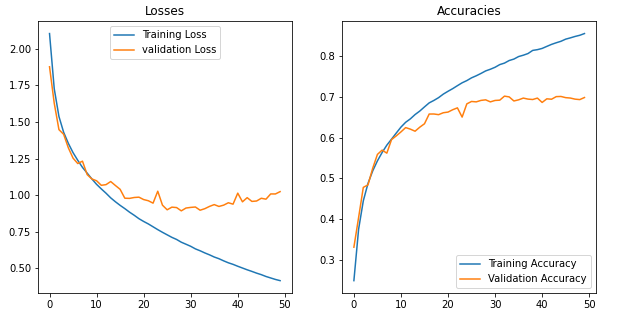
\includegraphics[scale = 0.35]{../images/cnn_model}
					\caption{Training of Convolutional Neural network}
					\label{fig:cnn}
				\end{subfigure}
			\caption{Training of linear classifier and CNN}
			\end{figure}
	\section{Two Layer Neural Network}
		A two layer neural network with sigmoid function as the activation function for the hidden layer has been implemented. There is no activation at the output layer and loss is MSE. 
		\subsection{Model}
			As the hidden layer has 200 units, the weights have been initialized with the shapes of [(200, 3072), (200,1)] and [(10,200), (10,1)] for each layer 1 and 2 respectively. The code is similar to the linear classifier in listing \ref{backprop}.
			\begin{multicols}{2}
				\noindent
				\begin{align*}
					z_1 & = w_1X + b_1\\
					A_1 &= sigmoid(z1) \\
				\end{align*}
				\begin{align*}
					\hat{Y} & = w_2A_1 + b_2 \\
					L &= \frac{1}{m}\sum{(\hat{Y}-Y)^2}  
				\end{align*}
			\end{multicols}
		the derivatives related to each weight can be represented as follows using chain rule,
		\begin{multicols}{2}
			\noindent
			\begin{align*}
				\frac{dL}{d\hat{Y}} &= \frac{2}{m}(\hat{Y} - Y) \\
				\frac{dL}{db_2} &= \frac{dL}{d\hat{Y}}\\
				\frac{dL}{dA_1} &= w_2^T\frac{dL}{d\hat{Y}}\\
			\end{align*}
			\begin{align*}
				\frac{dL}{dz_1} &= \frac{dL}{dA_1} \times (A_1 * (1-A_1))\\
				\frac{dL}{dw_1} &= \frac{dL}{dz_1}X^T\\
				\frac{dL}{db_1} &= \frac{dL}{dz_1}\\
			\end{align*}
		\end{multicols}
		Gradient descent algorithm has been implemented with these gradients.
		\subsection{Results}
		This 2 layer model should perform better than the linear classifier in question 1. But since we are only training the network for 300 epochs the training and testing losses tends to be higher than the linear classifier. Training for more epochs will result in a better results.
		\begin{table}
			\centering
			\begin{tabular}{|c|c|}
				\hline
				Hyperparameters & Value \\
				\hline
				Initial Learning rate & 0.015 \\
				decay	& 0.005 \\
				\hline
			\end{tabular}
			\label{param2}
			\caption{Hyperparameters for two layer network in question 2 and 3}
		\end{table}
		\begin{table}
			\centering
			\begin{tabular}{|c|c|c|c|c|}
				\hline
				epoch & Training Loss & Training accuracy & Testing loss & Testing accuracy\\
				\hline
				1 & 0.99 & 10.00 & 0.92 & 8.56 \\
				300 & 0.8583 & 26.67 & 0.8573 & 27.04\\
				\hline
			\end{tabular}
			\caption{Training and testing loss and accuracy for 2 layer network}
			\label{nn2}
		\end{table}
	\section{Implementing Stochastic Gradient Descent}
		The disadvantage of gradient descent algorithm is it waits until all the training data is used for one gradient calculation and then makes a progress. Stochastic Gradient Descent(SGD) update gradients for every sample processed. Which makes use of all the computations carried out and makes process towards reducing loss from step 1. But this introduces fluctuation in training. Mini batches are used to solve this and helps to arrive at a converging point much faster than regular gradient descent. This can be observed by comparing losses and accuracies provided in table \ref{nn2} and table \ref{sgd}. 
		\subsection{Results}
		It can be observed that SGD with minibatch outperforms regular gradient descent by a huge margin with given number of epochs. But using SGD somewhat increases the runtime of training but provides better results. SGD is useful when there is high number of training samples are available. 
		\par
		After implementing SGD 2 layer network is trained better than the linear classifier on 300th epoch which regular gradient descent algorithm would have required more epochs or a higher learning rate. But SGD have optimized the model better with the same epochs and same learning rate.
		\begin{table}
			\centering
			\begin{tabular}{|c|c|c|c|c|}
				\hline
				epoch & Training Loss & Training accuracy & Testing loss & Testing accuracy\\
				\hline
				1 & 0.8967 & 13.62 & 0.8973 & 14.95 \\
				300 & 0.7635 & 43.08 & 0.7713 & 41.50\\
				\hline
			\end{tabular}
			\caption{Training and testing loss and accuracy for 2 layer network with SGD optimizer}
			\label{sgd}
		\end{table}
	\begin{figure}[h]
		\begin{subfigure}{0.45\linewidth}
			\centering
			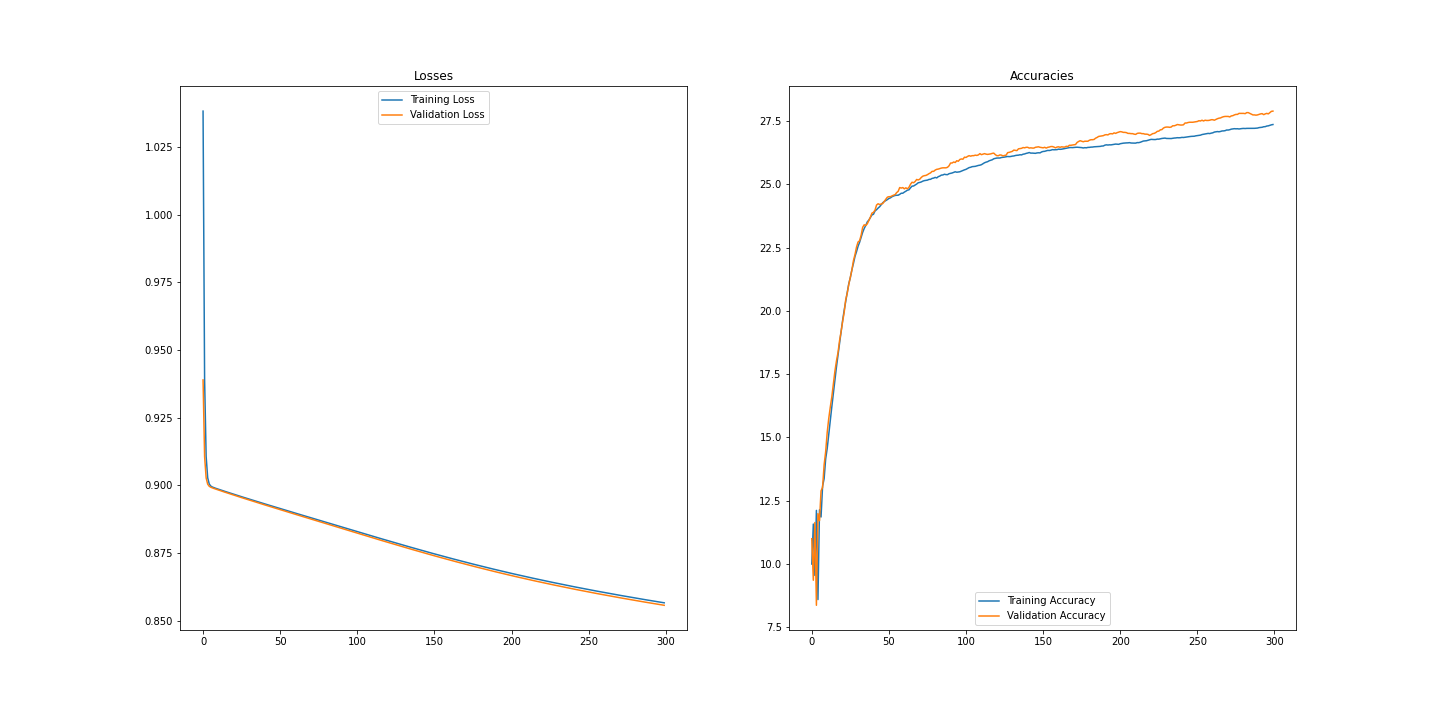
\includegraphics[scale = 0.35]{../images/two_layer_nn}
			\caption{Training of 2 layer neural network with gradient descent algorithm}
			\label{fig:nn2}
		\end{subfigure}
		\hfill
		\begin{subfigure}{0.45\linewidth}
			\centering
			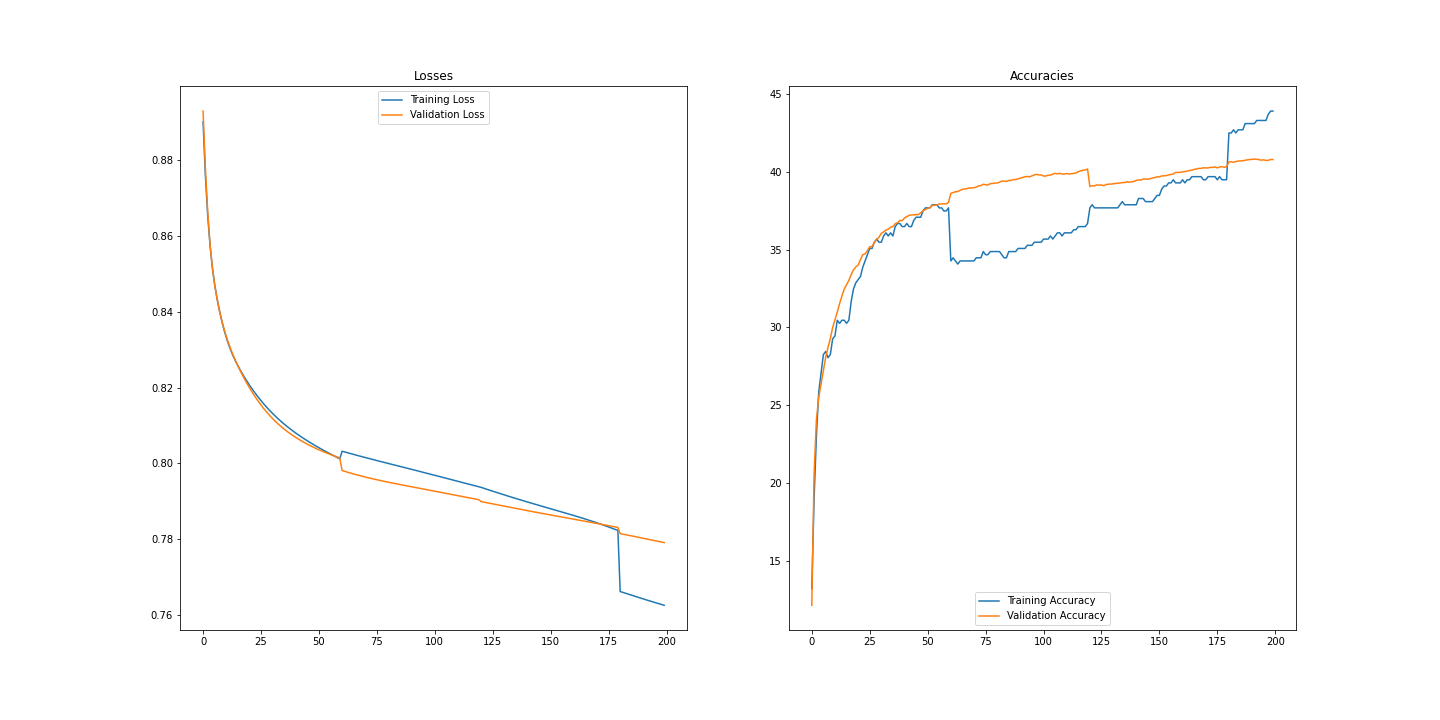
\includegraphics[scale = 0.35]{../images/two_layer_nn_sgd}
			\caption{Training of 2 layer neural network with Stochastic gradient descent algorithm}
			\label{fig:nn2sgd}
		\end{subfigure}
		\caption{Training with gradient descent and SGD}
	\end{figure}
	\section{Convolutional Neural Network with Keras}
		A Convolutional Neural network(CNN) has been implemented with the given architecture. Relu is used as activation for the convolutional layers and penultimate fully connected layer. Softmax function is used as the activation function of the last layer. SGD has been implemented with learning rate \textbf{0.01} and momentum \textbf{ 0.01}. 
		\par 
		As the convolutional layers extract features from the image, CNN outperform every network implemented from question 1 to 3. The results are provided in table \ref{cnn_la}. The implemented CNN passes the training loss and accuracy of 2 layer network with a small number of epochs. But it overfits the training data hence the testing loss is increasing after several number of epochs.
		\begin{table}[h]
			\centering
			\begin{tabular}{|c|c|c|c|c|}
				\hline
				epoch & Training Loss & Training accuracy & Testing loss & Testing accuracy\\
				\hline
				1 & 2.22 & 0.20 & 1.87 & 0.33 \\
				50 & 0.41 & 0.85 & 1.02 & 0.69\\
				\hline
			\end{tabular}
			\caption{Training and testing loss and accuracy for CNN model}
			\label{cnn_la}
		\end{table}
		\subsection{Number of learnable parameters}
			Maxpooling layers and flatten layer has no parameters. The number of parameters in a convolutional layer  can be calculated as shown in equation \ref{cnn_p}
			\begin{equation}
				n_i = [(h \times w \times f_{i-1}) + 1] \times f_i
				\label{cnn_p}
			\end{equation}
			here $h,w$ are the height and width of the filter. $f_i$ is the number of filters in layer $i$. 1 is added for the bias term of each filter. Using equation \ref{cnn_p} the calculated numbers are shown in table \ref{cnn_paramters}. 
			\begin{table}[h]
				\centering
				\begin{tabular}{|c|c|c|}
					\hline
					Layer & Parameter calculation & Number of parameters \\
					\hline
					Layer 1: C32 & [$(3\times 3\times 3\times)+1]\times 32$ & 896 \\
					Layer 2: C64 & [$(3\times 3\times 32\times)+1]\times 64$ & 18496 \\
					Layer 3: C64 & [$(3\times 3\times 64\times)+1]\times 64$ & 36928 \\
					Layer 4: F64 & $256 \times 64 + 64$ & 16448\\
					Layer 5: F10 & $64 \times 10 + 10$ & 650\\
					\hline
					Total parameters & & 73418\\
					\hline
				\end{tabular}
				\caption{Number of parameters in the CNN model}
				\label{cnn_paramters}
			\end{table}
			
			
\end{document}